\documentclass[../TDE6_rsf.tex]{subfiles}%

\begin{document}
\section[s]"2"{Comportement d'un circuit à haute et basse fréquence}
\enonce{%
	\noindent
	\begin{minipage}[t]{.6\linewidth}
		On considère le circuit ci-contre. On pose $e(t) = E_m\cos(\wt)$ et $u(t) =
			U_m\cos(\wt+\f)$.
	\end{minipage}
	\hfill
	\begin{minipage}{0.35\linewidth}
		\begin{center}
			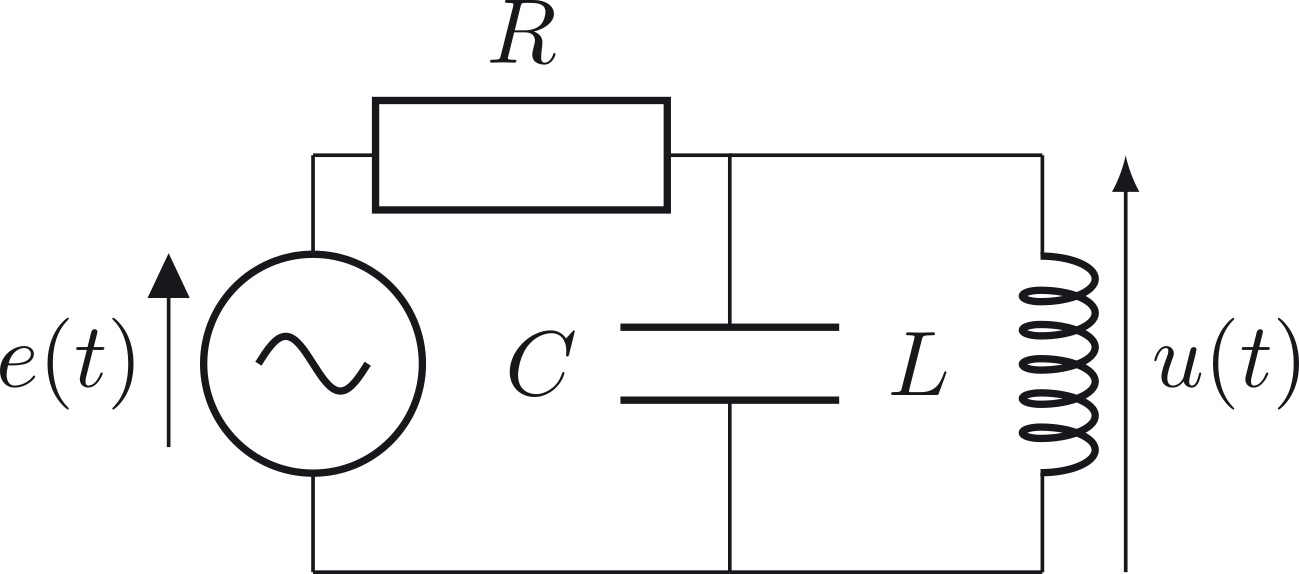
\includegraphics[width=\linewidth]{exo4_plain}
		\end{center}
	\end{minipage}
}

\QR{%
	Définir les signaux complexes $\xul{e}(t)$ et $\xul{u}(t)$ puis les
	amplitudes complexes $\Eu$ et $\Uu$ associées aux tensions
	$e(t)$ et $u(t)$, respectivement.
}{%
	On utilise la relation pour passer des réels aux complexes, pour avoir
	\[
		\boxed{\xul{e}(t) = E_m\exr^{\jwt}}
		\qet
		\boxed{\xul{u}(t) = U_m\exr^{\jj(\wt+\f)}}
	\]
	Pour avoir les amplitudes complexes, on sépare le terme en $\wt$ du
	terme de phase~: on trouve donc
	\[
		\boxed{\Eu = E_m}
		\qet
		\boxed{\Uu = U_m\exr^{\jj\f}}
	\]
}

\QR{%
	Établir l'expression de $\Uu$ en fonction de $E_m$, $R$, $L$,
	$C$ et $\w$.
}{%

	S'il n'y avait pas la capacité, on pourrait facilement utiliser un pont
	diviseur de tension pour exprimer $\xul{u}$ en fonction de $\xul{e}$,
	$\Zu_R$ et $\Zu_L$. Pour se ramener à la situation du pont diviseur de
	tension, on détermine donc une première impédance équivalente issue de
	l'association en parallèle de $L$ et $C$, après les avoir converties en
	complexes. \bigbreak
	On peut déterminer $\Zu\ind{eq, 1}$ avec les admittances $\Yu_L = 1/\jj
		L \w$ et $\Yu_C = \jj C\w$, et utiliser le pont diviseur de tension
	directement avec l'amplitude complexe~: $\Uu =
		\frac{\Zu\ind{eq,1}}{\Zu\ind{eq,1}+\Zu_R}E_m$. Ainsi,
	\begin{gather*}
		\Uu = \frac{\dfrac{1}{
				\color{orange}\cancel{\dfrac{1}{\jj L\w} + \jj C\w}}}
		{\dfrac{1}{\textcolor{orange}{\cancel{\dfrac{1}{\jj L\w} + \jj C\w}}}
			+ R\color{orange}(…)}E_0
		\times \textcolor{orange}{
			\frac{\jj C\w + \dfrac{1}{\jj L\w}}{\jj C\w + \dfrac{1}{\jj L\w}}}
		\Lra
		\Uu = \frac{1}{1 + \jrcw + \dfrac{R}{\jj L\w}}E_0\\
		\Lra
		\boxed{
			\Uu = \frac{E_0}{1 + \jj \left( RC\w - \dfrac{R}{L\w} \right)}
		}
	\end{gather*}
	où on a simplifié la fraction en multipliant par le terme orange d'abord,
	puis en utilisant que $1/\jj = -\jj$.
}

\QR{%
	En déduire les expressions de $U_m$ et de $\f$ en fonction de
	$E_m$, $R$, $L$, $C$ et $\w$.
}{%
	On trouve l'amplitude réelle en prenant le module de l'amplitude
	complexe, et la phase en en prenant l'argument~:
	\begin{gather*}
		U_m
		= \abs{ \Uu }
		\Lra
		\boxed{U_m
			= \frac{E_m}{\sqrt{1 + \left( RC\w - \dfrac{R}{L\w} \right)^2}}
		}\\
		\f
		= \underbrace{\cancel{\arg(E_m)}}_{=0}
		- \arg \left( 1 + \jj \left( RC\w - \dfrac{R}{L\w} \right) \right)
		\Lra
		\tan\f = - \frac{RC\w - \dfrac{R}{L\w}}{1}\\
		\Lra
		\boxed{\f = \arctan \left( RC\w - \frac{R}{L\w} \right)}
	\end{gather*}
}

\QR{%
	Déterminer les valeurs limites de $U_m$ à très basse et très haute
	fréquence. Ces résultats étaient-ils prévisibles par une analyse
	qualitative du montage~?
}{%
	À très haute fréquence, i.e.\ $\w\ra\infty$, le dénominateur
	de l'amplitude réelle tend vers l'infini à cause du terme $RC\w$, donc
	l'amplitude vers 0~; c'est la même chose à très basse fréquence, i.e.\
	$\w\ra0^+$~: le dénominateur tend vers l'infini et l'amplitude
	vers 0, mais cette fois à cause du terme en $\dfrac{R}{L\w}$. On a donc
	\[
		\boxed{U_m \xrightarrow[\w\ra\infty]{} 0}
		\qet
		\boxed{U_m \xrightarrow[\w\ra0^+]{} 0}
	\]
	On pouvait prévoir ces résultats par l'étude directe du montage et des
	impédances en jeu~: en effet,
	\begin{align*}
		\Zu_C
		= \frac{1}{\jj C\w}
		\ra
		\abs{\Zu_C} \xrightarrow[\w\ra0]{} \infty
		 & \qet
		\abs{\Zu_C} \xrightarrow[\w\ra\infty]{} 0 \\
		\Zu_L
		= \jj L\w
		\ra
		\abs{\Zu_L} \xrightarrow[\w\ra0]{} 0
		 & \qet
		\abs{\Zu_L} \xrightarrow[\w\ra\infty]{} \infty
	\end{align*}
	Dans les deux cas, le circuit équivalent est l'association en série
	d'une résistance avec une association en parallèle d'un interrupteur
	ouvert et d'un fil, c'est-à-dire un fil~: or, la tension d'un fil est
	nulle.
}
\end{document}
